\documentclass[18pt]{beamer}
\usepackage[utf8]{inputenc} % for the umlauts
\usepackage{subfigure}

\beamertemplatenavigationsymbolsempty
%% SLIDE FORMAT

% use 'beamerthemekit' for standard 4:3 ratio
% for widescreen slides (16:9), use 'beamerthemekitwide'

\usepackage{templates/beamerthemekit}
% \usepackage{templates/beamerthemekitwide}

\setcounter{tocdepth}{1}

%% TITLE PICTURE

% if a custom picture is to be used on the title page, copy it into the 'logos'
% directory, in the line below, replace 'mypicture' with the 
% filename (without extension) and uncomment the following line
% (picture proportions: 63 : 20 for standard, 169 : 40 for wide
% *.eps format if you use latex+dvips+ps2pdf, 
% *.jpg/*.png/*.pdf if you use pdflatex)

%\titleimage{mypicture}

%% TikZ INTEGRATION

% use these packages for PCM symbols and UML classes
% \usepackage{templates/tikzkit}
% \usepackage{templates/tikzuml}

% the presentation starts here

\usepackage{mathabx}
\usepackage{picture}
\usepackage[absolute,overlay]{textpos}
%\usepackage[texcoord,grid,gridunit=mm,gridcolor=red, subgridcolor=green]{eso-pic}
\setbeamercovered{invisible}
\setbeamertemplate{caption}{\raggedright\insertcaption\par}

\title[SWT1]{Softwaretechnik 1 - 4. Tutorium}
\subtitle{Tutorium 03}
\author{Felix Bachmann}
\date{26.06.2017}

\institute{KIT - Institut für Programmstrukturen und Datenorganisation (IPD)}

% Bibliography

\usepackage[citestyle=authoryear,bibstyle=numeric,hyperref,backend=biber]{biblatex}
\addbibresource{templates/example.bib}
\bibhang1em

\begin{document}

% change the following line to "ngerman" for German style date and logos
\selectlanguage{ngerman}

%title page
\begin{frame}
\titlepage
\end{frame}


\section{Orga}

	%TODO add design patterns extra slides (weekend)

	\subsection{Feedback 4. Übungsblatt}
	\begin{frame}
		%TODO
		\frametitle{4. Übungsblatt Statistik}
		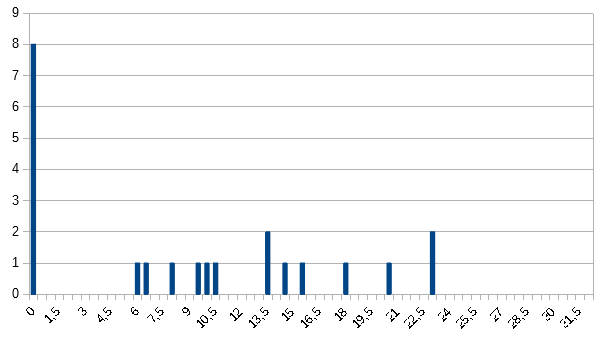
\includegraphics[scale=0.7]{./pics/tut4/statistics-ub4.png}
		\linebreak \centering $\diameter$ 6,45 bzw. 10,33 von (bisher) 15+1
	\end{frame}
	
	\subsection{4. Übungsblatt - Fehler (Allgemein)}
	\begin{frame}
		%TODO
		\frametitle{Häufige Fehler}
		\begin{block}{Allgemein}
			\begin{itemize}
				\item Form bei handschriftlichen Abgaben\dots
			\end{itemize}
		\end{block}
	\end{frame}
	
	\subsection{4. Übungsblatt - Fehler}
	\begin{frame}
		\frametitle{Häufige Fehler}
		%TODO
		\begin{block}{Aufgabe 1 (Zustandsdiagramm - LEZ): $\diameter$ 2,81 bzw. 4,5 von 5+1}
			\begin{itemize}
				\pause 
				\item Hierarchie sinnvoll, wenn aus mehreren Zuständen gleiche Übergänge in den gleichen Zustand gehen \pause
				\item nach VL gibt es im Zustandsdiagramm kein "'Karo"' \pause
				\item "'Versehen Sie die Zustandsübergänge mit Ereignissen \textbf{und} Operationen."' \pause
				\linebreak $\implies$ kann in Klausur bei Nichtbeachtigung Punktabzug geben
			\end{itemize}
		\end{block}
	\end{frame}

	\begin{frame}
		\frametitle{Häufige Fehler}
		%TODO
		\begin{block}{Aufgabe 2 (Abbottsche Methode): $\diameter$ 1,73 bzw. 3,19 von 5}
			\begin{itemize}
				\pause 
				\item bei "'auseinandergezogenen Verben"' alle Teile des Verbs markieren \pause
				\linebreak z.B "'teilnehmen"' $\implies$ "'Studenten nehmen an VL teil"' \pause
				\item Worte kommen mehrfach vor $\implies$ jedes Mal markieren! \pause
				\item bei jedem "'ist"', "'sind"', etc. Vererbung \pause
				\item "'wissenschaftlicher Mitarbeiter"' = Attribut und Klasse
			\end{itemize}
		\end{block}
		\pause 
		%TODO
		\begin{block}{Aufgabe 3 (iMage-GUI): $\diameter$ (tbd)}
			\begin{itemize}
				\item	(nächstes Mal)
			\end{itemize}
		\end{block}
	\end{frame}

	\begin{frame}
		\frametitle{Häufige Fehler}
		%TODO
		\begin{block}{Aufgabe 4 (Geheimnisprinzip): $\diameter$ 1,92 bzw. 3,07 von 5}
			\begin{itemize}
				\pause
				\item nicht nur die öffentlichen Konstanten sind problematisch, sondern auch die getter und setter \pause
				\linebreak $\implies$ die Entscheidung den Zustand intern als int zu repräsentieren muss versteckt werden \pause 
				\linebreak $\implies$ nach außen immer boolean benutzen (wohldefiniert!)
			\end{itemize}
		\end{block}
	\end{frame}

\section{Recap}
	\subsection{Quiz(Adapter)}
	\begin{frame}
		\frametitle{Was bisher geschah..}
		\begin{itemize}
			\item haben uns erste Entkopplungmuster angeschaut \pause
			\linebreak $\implies$ Beobachter, Iterator, Adapter, Stellvertreter, Vermittler \pause
		\end{itemize}
		\begin{figure}
			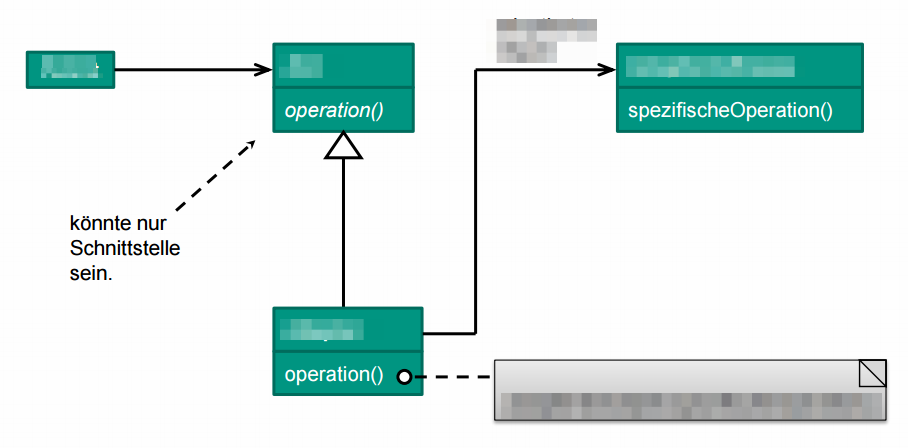
\includegraphics[scale=0.33]{./pics/tut4/adap-obj-mod.png}
		\end{figure}
		Welches Entwurfsmuster? \pause (Objekt-)Adapter
	\end{frame}
	
	\begin{frame}
		\frametitle{Was bisher geschah..}
		\begin{itemize}
			\item haben uns erste Entkopplungmuster angeschaut
			\linebreak $\implies$ Beobachter, Iterator, Adapter, Stellvertreter, Vermittler
		\end{itemize}
		\begin{figure}
			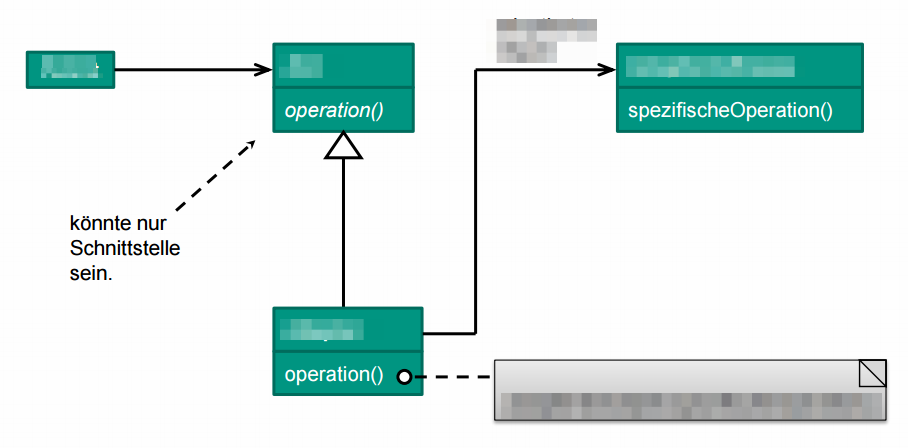
\includegraphics[scale=0.33]{./pics/tut4/adap-obj-mod.png}
		\end{figure}
		Welche Klassen?
	\end{frame}
	
	\begin{frame}
		\frametitle{Was bisher geschah..}
		\begin{itemize}
			\item haben uns erste Entkopplungmuster angeschaut
			\linebreak $\implies$ Beobachter, Iterator, Adapter, Stellvertreter, Vermittler
		\end{itemize}
		\begin{figure}
			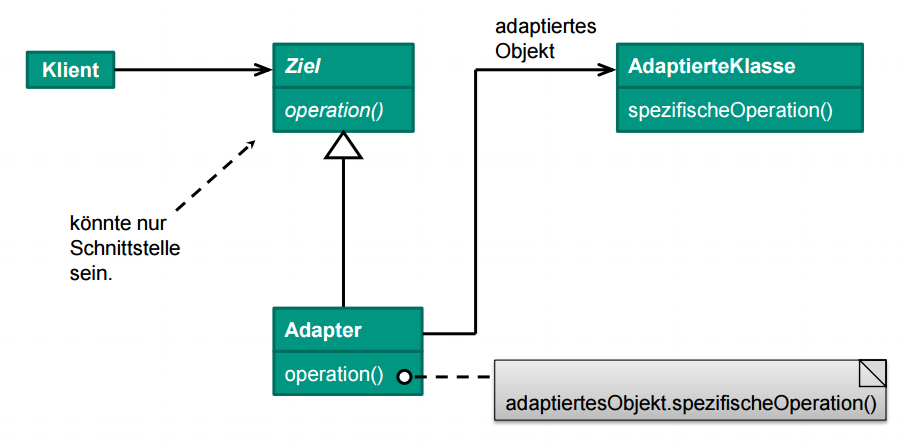
\includegraphics[scale=0.45]{./pics/tut3/adap-obj.png}
		\end{figure}
	\end{frame}
	
	\subsection{Quiz (Iterator)}
	\begin{frame}
		\frametitle{Was bisher geschah..}
		\begin{itemize}
			\item haben uns erste Entkopplungmuster angeschaut
			\linebreak $\implies$ Beobachter, Iterator, Adapter, Stellvertreter, Vermittler
		\end{itemize}
		\begin{figure}
			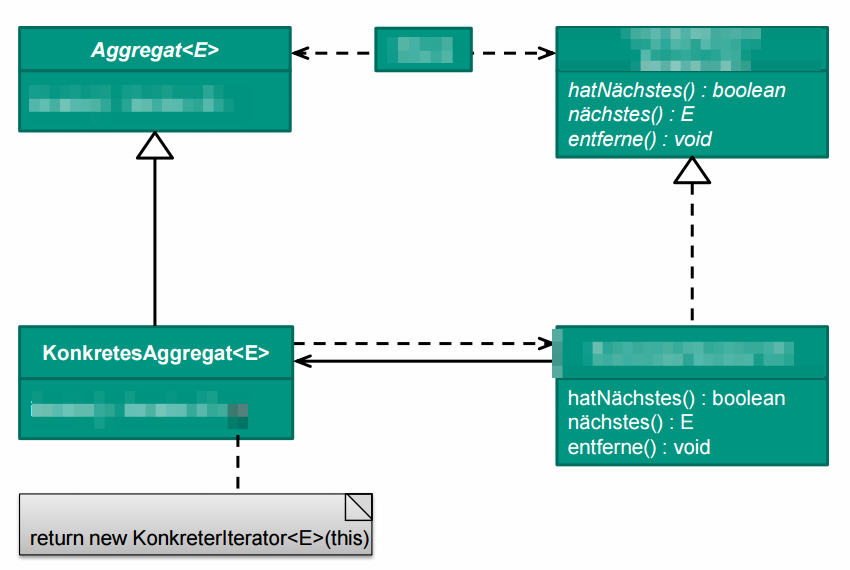
\includegraphics[scale=0.25]{./pics/tut4/iter-mod.png}
		\end{figure}
		Welches Entwurfsmuster? \pause Iterator
	\end{frame}
	
	\begin{frame}
		\frametitle{Was bisher geschah..}
		\begin{itemize}
			\item haben uns erste Entkopplungmuster angeschaut
			\linebreak $\implies$ Beobachter, Iterator, Adapter, Stellvertreter, Vermittler
		\end{itemize}
		\begin{figure}
			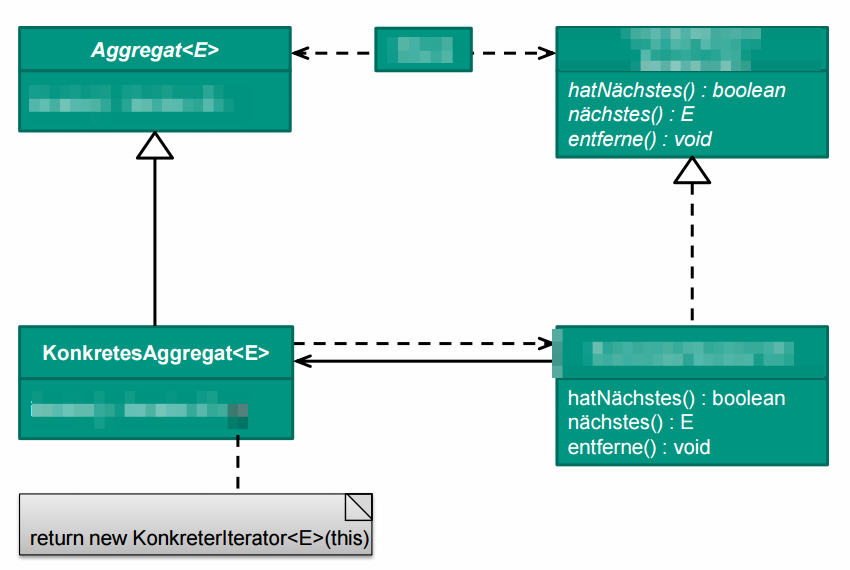
\includegraphics[scale=0.25]{./pics/tut4/iter-mod.png}
		\end{figure}
		Welche Klassen und Methoden?
	\end{frame}
	
	\begin{frame}
		\frametitle{Was bisher geschah..}
		\begin{itemize}
			\item haben uns erste Entkopplungmuster angeschaut
			\linebreak $\implies$ Beobachter, Iterator, Adapter, Stellvertreter, Vermittler
		\end{itemize}
		\begin{figure}
			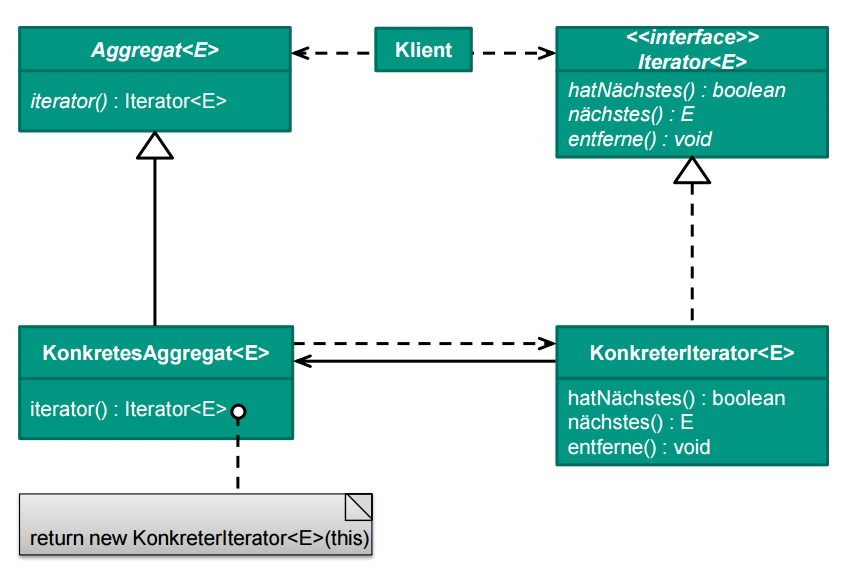
\includegraphics[scale=0.35]{./pics/tut3/iter.png}
		\end{figure}
	\end{frame}
	
	\subsection{Quiz(Beobachter)}
	
	\begin{frame}
		\frametitle{Was bisher geschah..}
		\begin{itemize}
			\item haben uns erste Entkopplungmuster angeschaut
			\linebreak $\implies$ Beobachter, Iterator, Adapter, Stellvertreter, Vermittler
		\end{itemize}
		\begin{figure}
			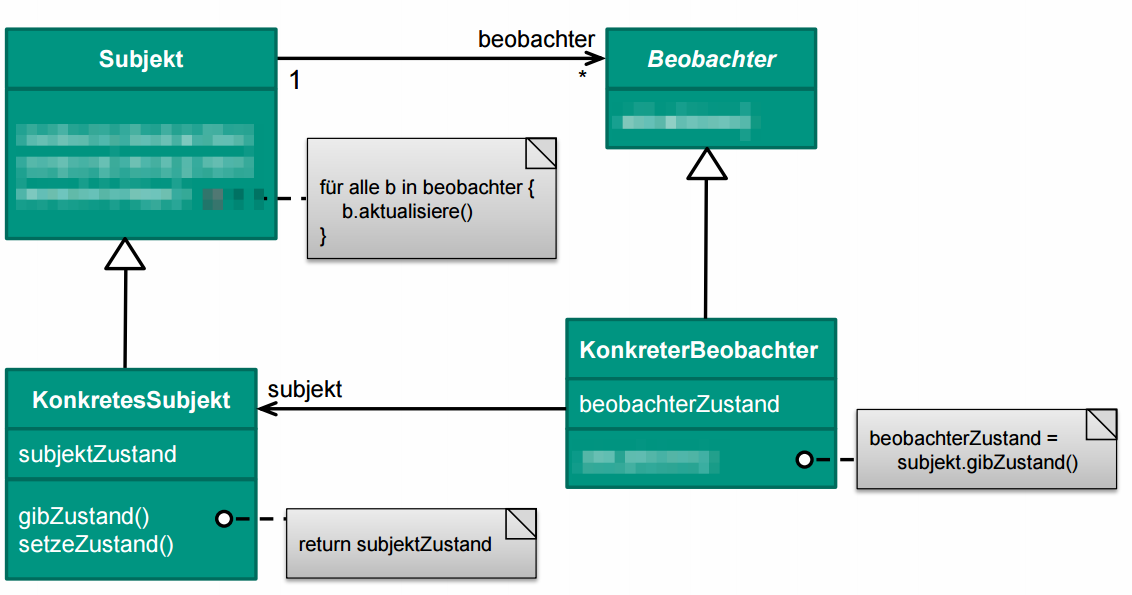
\includegraphics[scale=0.25]{./pics/tut4/obs-mod.png}
		\end{figure}
		\pause Ist wohl ein Beobachter :) \pause Methoden?
	\end{frame}
	
	\begin{frame}
		\frametitle{Was bisher geschah..}
		\begin{itemize}
			\item haben uns erste Entkopplungmuster angeschaut
			\linebreak $\implies$ Beobachter, Iterator, Adapter, Stellvertreter, Vermittler
		\end{itemize}
		\begin{figure}
			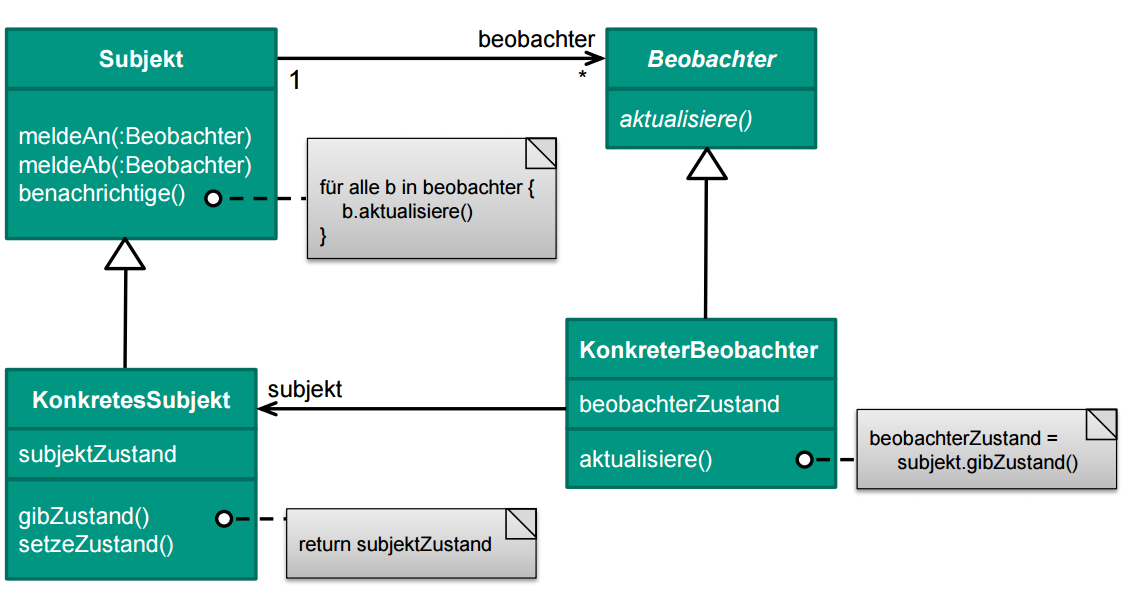
\includegraphics[scale=0.35]{./pics/tut3/obs.png}
		\end{figure}
	\end{frame}

	%TODO Stellvertreter, Vermittler recap

	\begin{frame}
		\frametitle{Kategorien der Entwurfsmuster}
		\begin{itemize}
			\item \textbf{Entkopplungs-Muster}
			\begin{itemize}
				\item Adapter \colorbox{green}{fertig}
				\item Beobachter\colorbox{green}{fertig}
				\item Iterator \colorbox{green}{fertig}
				\item Stellvertreter \colorbox{green}{fertig}
				\item Vermittler \colorbox{green}{fertig}
				\item (Brücke)
			\end{itemize}
			\item Varianten-Muster
			\item Zustandshandhabungs-Muster
			\item Steuerungs-Muster
			\item Bequemlichkeits-Muster
		\end{itemize}
	\end{frame}

\section{Gruppenarbeit}
\subsection{Gruppenarbeit}
	\begin{frame}
		\frametitle{Kategorien der Entwurfsmuster}
		\begin{itemize}
			\item Entkopplungs-Muster \colorbox{green}{fertig}
			\item \textbf{Varianten-Muster}
			\begin{itemize}
				\item (Abstrakte Fabrik)
				\item (Besucher)
				\item \textbf{Schablonenmethode}
				\item \textbf{Fabrikmethode}
				\item \textbf{Kompositum}
				\item Strategie \colorbox{green}{fertig}
				\item \textbf{Dekorierer}
			\end{itemize}
			\item Zustandshandhabungs-Muster
			\item Steuerungs-Muster
			\item Bequemlichkeits-Muster
		\end{itemize}
	\end{frame}
	
	\begin{frame}
		\frametitle{Varianten-Muster}
		\begin{block}{Übergeordnetes Ziel}
			\begin{itemize}
				\item Gemeinsamkeiten herausziehen und an einer Stelle beschreiben \pause
				\linebreak $\implies$ keine Wiederholung desselben Codes \pause
				\linebreak $\implies$ bessere Wartbarkeit/Erweiterbarkeit		
			\end{itemize}
		\end{block}
	\end{frame}
	
	\begin{frame}
		\frametitle{Jetzt: Gruppenarbeit}
		\begin{enumerate}
			\item ihr kriegt pro Reihe eine Aufgabe
			\item ihr habt Zeit zum Bearbeiten
			\item Abgleichung mit Musterlösung
			\item ihr stellt den anderen eure Lösung vor
		\end{enumerate}
	\end{frame}

	\begin{frame}
		\frametitle{Vorstellung Dekorierer}
		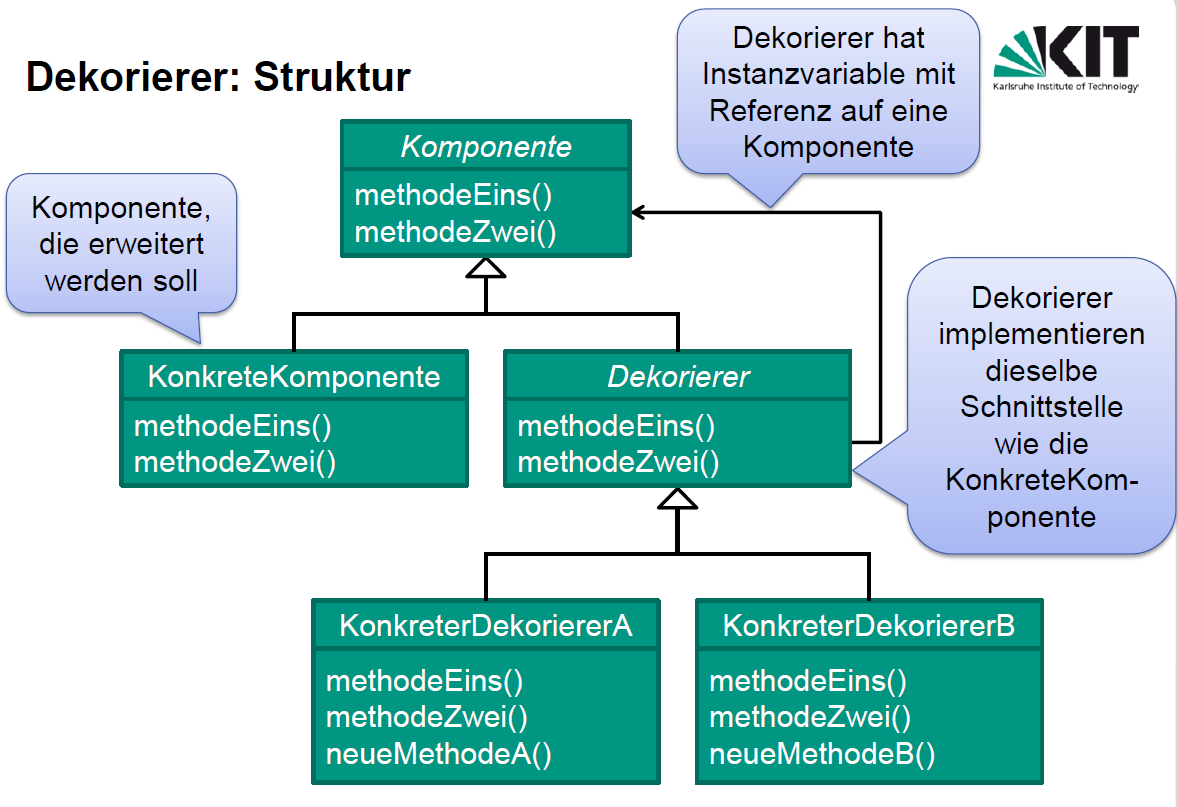
\includegraphics[scale=0.35]{./pics/tut4/decor.png}
	\end{frame}

	\begin{frame}
		\frametitle{MuLö Dekorierer}
		\begin{block}{Wo Gemeinsamkeiten?}
			Die beiden Methoden methodeEins() und methodeZwei().
		\end{block}
		\begin{block}{Wo Variation?}
			In den KonkretenDekorierern bzw. ihren Methoden. Hier: neueMethodeA(), neueMethodeB().
		\end{block}
		\begin{block}{Wozu Instanzvariable?}
			Weiterleitung von Aufrufen der methodeEins() und methodeZwei() an die KonkreteKompenente.
		\end{block}
	\end{frame}

	\begin{frame}
		\frametitle{Vorstellung Kompositum}
		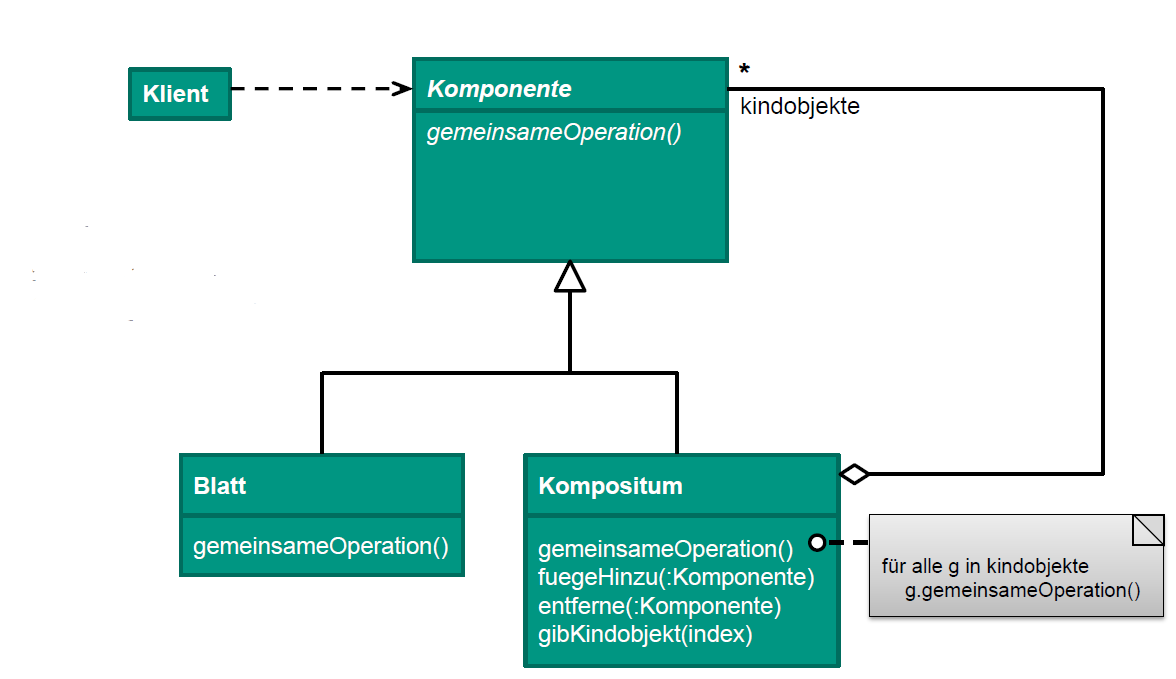
\includegraphics[scale=0.35]{./pics/tut4/comp.png}
	\end{frame}

	\begin{frame}
		\frametitle{MuLö Kompositum}
		\begin{block}{Wo Gemeinsamkeiten?}
			gemeinsameOperation().
		\end{block}
		\begin{block}{Wo Variation?}
			In Blatt/Kompositum-Klassen mit verschiedenen zusätzlichen Operationen.
		\end{block}
		\begin{block}{Zusammengesetzt vs. nicht-zusammengesetzt}
			Kompositum = zusammengesetzt, Blatt = nicht-zusammengesetzt
		\end{block}
	\end{frame}

	\begin{frame}
		\frametitle{Vorstellung Schablonenmethode}
		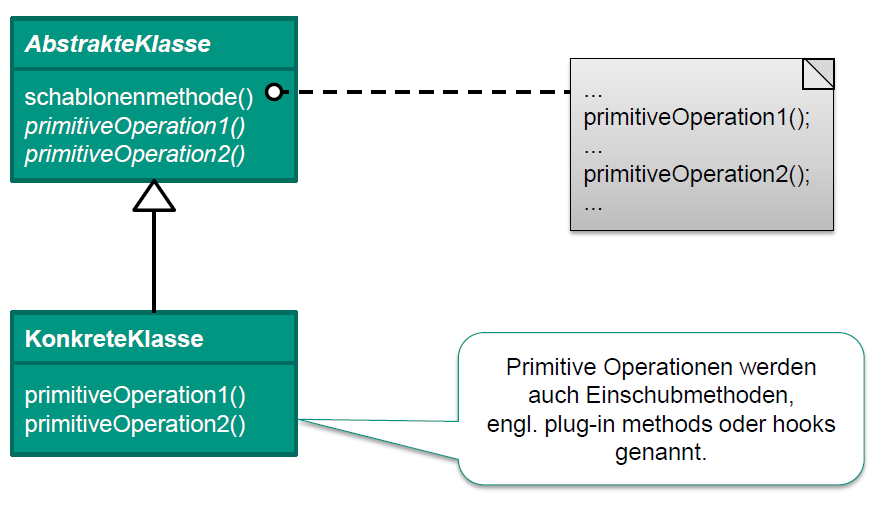
\includegraphics[scale=0.45]{./pics/tut4/schab.png}
	\end{frame}

	\begin{frame}
		\frametitle{MuLö Schablonenmethode}
		\begin{block}{Wo Gemeinsamkeiten?}
			Reihenfolge der Methodenaufrufe in der Schablonenmethode.
		\end{block}
		\begin{block}{Wo Variation?}
			In den Einschubmethoden. (hier: primitiveOperation1() und primitiveOpoeration2())
		\end{block}
		\begin{block}{Schablonenmethode vs. Einschubmethode}
			Einschubmethode ist eine der Methoden, die von der Schablonenmethode aufgerufen wird und deren Implementierung in den Unterklassen stattfindet.
		\end{block}
	\end{frame}

	\begin{frame}
		\frametitle{Vorstellung Fabrikmethode}
		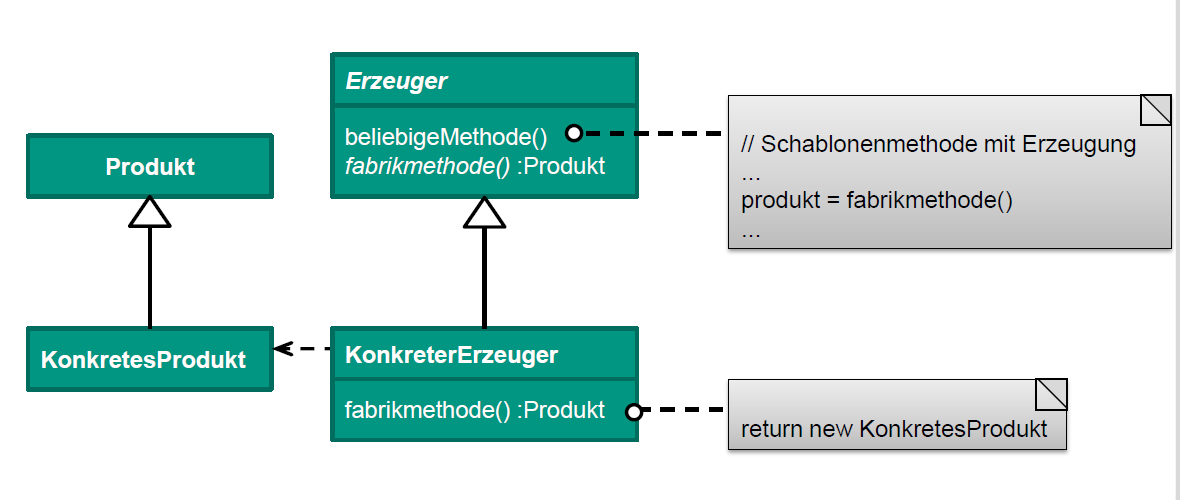
\includegraphics[scale=0.4]{./pics/tut4/fab.png}
	\end{frame}

	\begin{frame}
		\frametitle{MuLö Fabrikmethode}
		\begin{block}{Wo Gemeinsamkeiten?}
			Reihenfolge der Methodenaufrufe in der beliebigenMethode().
		\end{block}
		\begin{block}{Wo Variation?}
			In der Fabrikmethode.
		\end{block}
		\begin{block}{Klasse des Objekts, Oberklasse, Unterklasse}
			Klasse des Objekts = KonkretesProdukt, Oberklasse = Produkt, Unterklasse = KonkreterErzeuger
		\end{block}
		\begin{block}{Unterschied zu Schablonenmethode?}
			Fabrikmethode benutzen, wenn ein Objekt erzeugt wird. Fabrikmethode ist Einschubmethode des Musters "'Schablonenmethode"'.
		\end{block}
		\begin{block}{Wahr/falsch}
			Fabrikmethode ist eine Einschubmethode, keine Schablonenmethode.
		\end{block}
	\end{frame}

\section{Memento}
	\subsection{Intro}
	\begin{frame}
		\frametitle{Kategorien der Entwurfsmuster}
		\begin{itemize}
			\item Entkopplungs-Muster \colorbox{green}{fertig}
			\item Varianten-Muster \colorbox{green}{fertig}
			\item \textbf{Zustandshandhabungs-Muster}
				\begin{itemize}
					\item (Einzelstück)
					\item (Fliegengewicht)
					\item \textbf{Memento} 
					\item (Prototyp) 
					\item (Zustand)
				\end{itemize}
			\item Steuerungs-Muster
			\item Bequemlichkeits-Muster
		\end{itemize}
	\end{frame}

	\begin{frame}
		\frametitle{Zustandshandhabungs-Muster}
		\begin{block}{Übergeordnetes Ziel}
			\begin{itemize}
				\item den Zustand eines Objektes beschreiben (wer hätt's gedacht? :D) \pause 
				\item aber unabhängig von dem Zweck des Objekts!
			\end{itemize}
		\end{block}
	\end{frame}

	%TODO singleton, zustand

	\begin{frame}
		\frametitle{Memento}
		\begin{block}{Problem}
			\begin{itemize}
				\item internen Zustand eines Objekts "'externalisieren"', um z.B. Zurücksetzen möglich zu machen \pause 
				\item ohne Kapselung zu verletzten!
			\end{itemize}
		\end{block}
		\pause
		\centering
		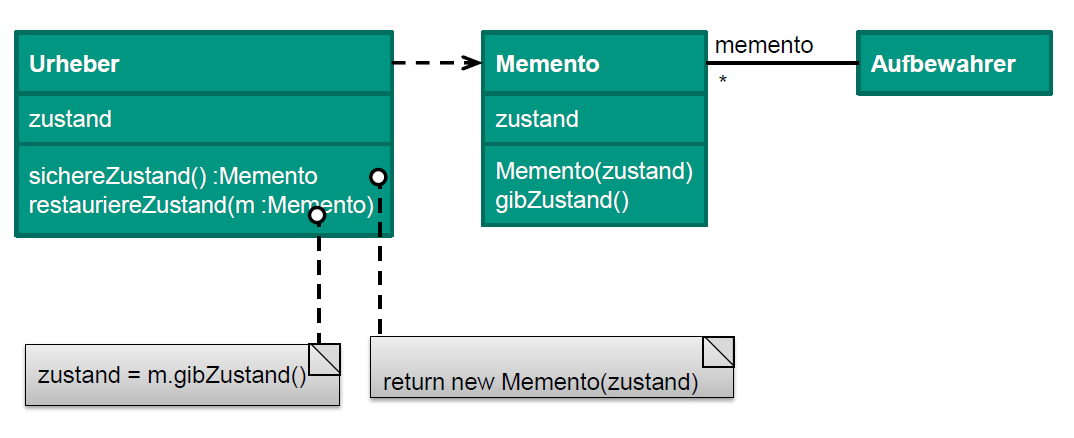
\includegraphics[scale=0.4]{./pics/tut4/mem.png}
	\end{frame}

	\begin{frame}
		\frametitle{Memento}
		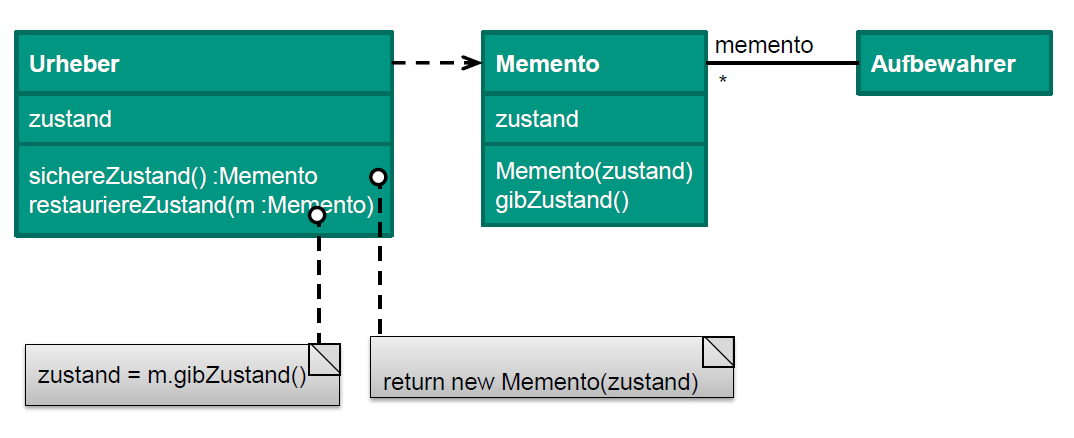
\includegraphics[scale=0.4]{./pics/tut4/mem.png}
		\begin{block}{Problem gelöst?}
			\begin{itemize}
				\pause
				\item Ja
				\begin{itemize}
					\pause
					\item Zustand durch Memento externalisiert \pause
					\item Kapselung nicht verletzt (Nutzer ruft nur sichereZustand() auf und kriegt neuen Memento)
				\end{itemize}
			\end{itemize}
		\end{block}
\end{frame}

\section{Befehl}
	\subsection{Intro}
	\begin{frame}
		\frametitle{Kategorien der Entwurfsmuster}
		\begin{itemize}
			\item Entkopplungs-Muster \colorbox{green}{fertig}
			\item Varianten-Muster \colorbox{green}{fertig}
			\item Zustandshandhabungs-Muster \colorbox{green}{fertig}
			\item \textbf{Steuerungs-Muster} 
				\begin{itemize}
					\item \textbf{Befehl}
					\item (master/worker)
				\end{itemize}
			\item Bequemlichkeits-Muster
		\end{itemize}
	\end{frame}
	
	\begin{frame}
		\frametitle{Steuerungs-Muster}
		\begin{block}{Übergeordnetes Ziel}
			\begin{itemize}
				\item steuern den Kontrollfluss \pause 
				\linebreak $\implies$ zur richtigen Zeit richtige Methoden aufrufen
			\end{itemize}
		\end{block}
	\end{frame}

	\begin{frame}
		\frametitle{Befehl}
		\begin{block}{Problem}
			\begin{itemize}
				\item Parametrisieren von Objekten mit einer auszuführenden Aktion \pause 
				\item komplexe Operationen aus primitiven Operationen aufbauen \pause
				\linebreak $\implies$ Befehl nicht als Methode, sondern als Objekt modellieren
			\end{itemize}
		\end{block}
		\pause
		\centering
		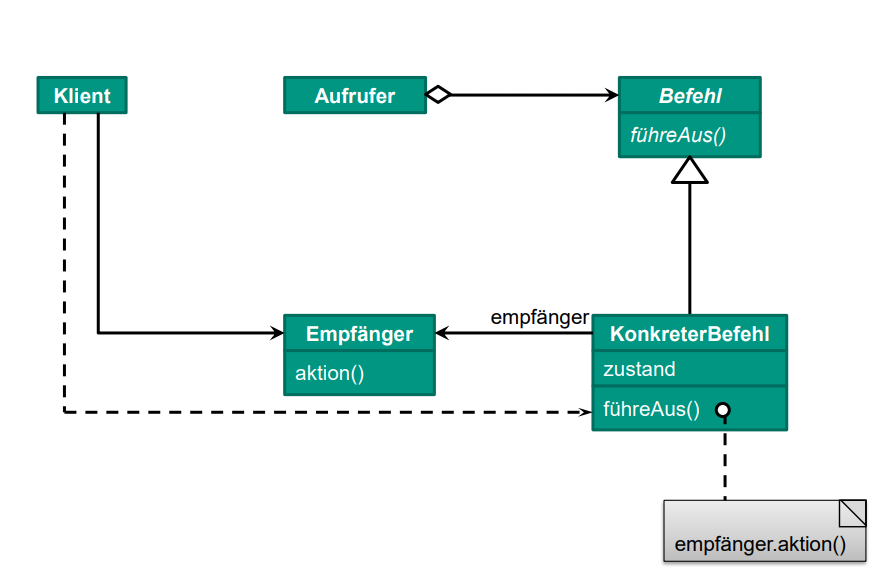
\includegraphics[scale=0.33]{./pics/tut4/command.png}
	\end{frame}

	\begin{frame}
		\frametitle{Befehl}
		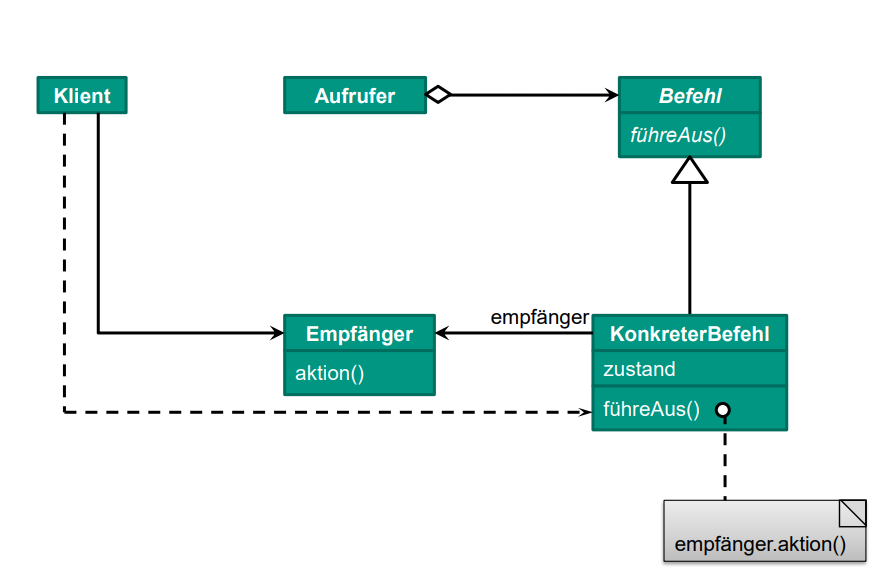
\includegraphics[scale=0.35]{./pics/tut4/command.png}
		\begin{block}{Was haben wir erreicht?}
			\begin{itemize}
				 \pause
				\item Austauschbarkeit: Befehle unabhängig vom Aufrufer, universell einsetzbar
			\end{itemize}
		\end{block}
	\end{frame}
	
	\begin{frame}
		\frametitle{Quiz (Ankreuzaufgaben aus Klausuren)}
		Wahr oder falsch?
		\begin{itemize}
			\item Bei dem Entwurfsmuster Befehl kennt der Empfänger den Befehl nicht, jedoch der Befehl den Empfänger. \pause \colorbox{green}{wahr} \pause
			\item Ein Aufbewahrer im Entwurfsmuster Memento kann beliebig viele Mementos verwalten. Für die Restauration im Falle eines Reset ist er allerdings nicht verantwortlich. \pause \colorbox{green}{wahr} \pause
			\item Die Fabrikmethode sorgt dafür, dass nur eine einzige Instanz einer Klasse fabriziert wird. \pause \colorbox{red}{falsch} \pause 
			\item Eine Schablonenmethode ist immer auch eine Fabrikmethode. \pause \colorbox{red}{falsch} \pause
			\item Eine Komponente kann immer nur mit einem einzigen Dekorierer versehen werden. \pause \colorbox{red}{falsch}
		\end{itemize}
	\end{frame}
	
	
	\begin{frame}
		\frametitle{Für die Klausur}
		\begin{itemize}
			\item Entwurfsmuster kommen sehr sehr sehr wahscheinlich dran! \pause 
			\item Kategorien helfen beim Lernen \pause
			\item jedes Entwurfsmuster erfüllt einen bestimmten Zweck 
			\linebreak $\implies$ nicht nur die Klassen und Methoden auswendig lernen, sondern das Prinzip verstehen \pause
			\item bei Unklarheiten in Head First Design Patterns nachlesen ;)
		\end{itemize}
	\end{frame}

\section{Feedback}
	\subsection{Feedback}
	\begin{frame}
		\frametitle{Feedback - Sagt mir eure Meinung}
		%TODO google docs oder so
		\begin{enumerate}
			\item nehmt einen Zettel
			\item schreibt (konstruktives!) Feedback darauf
			\begin{itemize}
				\item am besten $\geq$ 4 Stichpunkte
			\end{itemize}
			\item legt euren Zettel beim Rausgehen nach vorne
		\end{enumerate}
\end{frame}
	
\section{Tipps}
	\subsection{Tipps}
	\begin{frame}
		\frametitle{Tipps - 5. Übungsblatt}
			\begin{exampleblock}{Aufgabe 1: Manager-Deutsch und Architekturstile} 
				\begin{itemize}
					\item Architekturstile nochmal anschauen
				\end{itemize}
			\end{exampleblock}
			\pause
			\begin{exampleblock}{Aufgabe 2: Iterator für Plug-Ins} 
				\begin{itemize}
					\item Iterator-Muster selbst benutzen
				\end{itemize}
			\end{exampleblock}
	\end{frame}

	\begin{frame}
		\frametitle{Tipps - 5. Übungsblatt}
			\begin{exampleblock}{Aufgabe 3: Geometrify mit Entwurfsmustern}
				\begin{itemize}
					\item überlegen, welches Entwurfsmuster \textbf{warum} Sinn macht
				\end{itemize}
			\end{exampleblock}
			\pause
			\begin{exampleblock}{Aufgabe 4: Geometrify umstrukturieren}
				\begin{itemize}
					\item Überlegungen aus Aufgabe 3 umsetzen
				\end{itemize}
			\end{exampleblock}
	\end{frame}

	\begin{frame}
		\frametitle{Tipps - 5. Übungsblatt}
		\begin{exampleblock}{Aufgabe 5: GUI erweitern}
			\begin{itemize}
				\item nochmal ServiceLoader
			 	 $\implies$ diesmal mit Primitiven
			\end{itemize}
		\end{exampleblock}
	\end{frame}
	
	\subsection{Abgabe}
	\begin{frame}
		\frametitle{Denkt dran!}
		\begin{alertblock}{Abgabe}
			\begin{itemize}
				\item Deadline am 27.6. um 12:00
				\item Aufgabe 1, 3 handschriftlich (wirklich handschriftlich!)
			\end{itemize}
		\end{alertblock}
	\end{frame}
		
	\begin{frame}
		\frametitle{Bis dann! (dann  := 03.07.18)}
		\centering
		
\includegraphics[scale=0.4]{./comics/patterns.jpg}
	\end{frame}

\end{document}